\documentclass[a4paper]{sbgames}               % final
%\usepackage[scaled=.92]{helvet}

\usepackage[brazil]{babel}
\usepackage[latin1]{inputenc}


\usepackage{times}
\usepackage{graphicx}

%% use this for zero \parindent and non-zero \parskip, intelligently.
\usepackage{parskip}

%% the 'caption' package provides a nicer-looking replacement
\usepackage[labelfont=bf,textfont=it]{caption}

\usepackage{url}

%% Paper title.
\title{Um Sistema para Gera��o Procedural de Terrenos Pseudo-Infinitos em Tempo-Real Utilizando GPU e CPU}

%% Author and Affiliation (multiple authors). Use: and between authors

%\author{Name1 A. Surname1\\ Digital Games Lab 
%        \and Name2 B. Surname2\\ Name3 C. Surname3\\ ZZZZ University
%        \and Name4 D. Surname4\\ Farwest Research Center 
%}
%\contactinfo{\{name1,name3\}@xxx.yyyy.yyy \\
%             *name2@zzzz.vvvv.vvv
%}
\author{60334}

%% Keywords that describe your work.
\keywords{modelagem procedural; gpu; gpgpu; programa��o paralela}

%% Start of the paper
% Attention: As you need to insert EPS images in Postscript, 
% you need to insert PDF images into PDFs. 
% In the text, extensions cancbe omitted (latex use .eps, pdflatex get .pdf) 
% To convert them: epstopdf myimage.eps
\begin{document}

\teaser{
  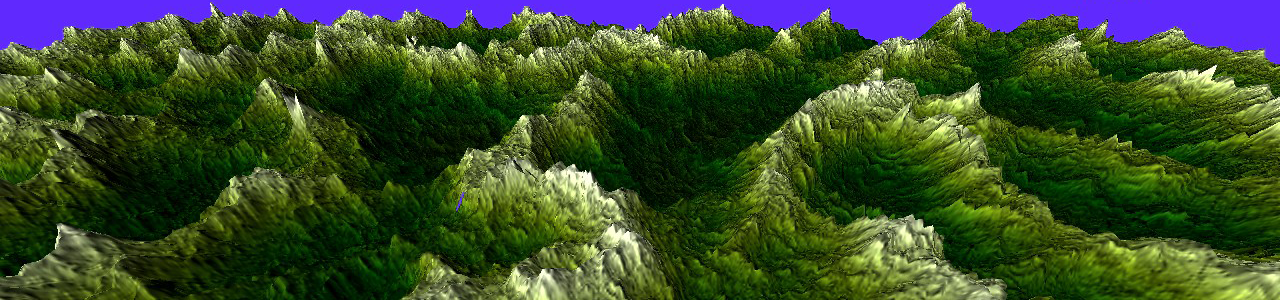
\includegraphics[width=.7\linewidth]{img/teaser.png}
  \caption{Terreno gerado proceduralmente.}
  \label{fig:teaser}
}

%% The ``\maketitle'' command must be the first command after the
%% ``\begin{document}'' command. It prepares and prints the title block.

\maketitle

%% Abstract section.

\begin{abstract}
O r�pido crescimento do poder de processamento das placas gr�ficas fez com que diversas tarefas migrassem da CPU para a GPU. Por�m, as unidades de processamento gr�fico podem ser vistas como aliadas da CPU, e n�o rivais. Este trabalho prop�e um sistema \emph{multithread} que utiliza tanto a CPU quanto a GPU para a gera��o procedural de terrenos, compartilhando a carga de trabalho entre as arquiteturas. Dessa forma, busca-se minimizar o tempo gasto com a gera��o e assim permitir uma navega��o fluida atrav�s de um mundo pseudo-infinito gerado proceduralmente.

Ao final, uma compara��o � feita com base em experimentos utilizando diferentes configura��es da arquitetura, com o objetivo de expor suas vantagens e aplica��es.
\end{abstract}

%% The ``\keywordlist'' command prints out the keywords.
\keywordlist
\contactlist

\chapter{INTRODUÇÃO}

\section{Visão geral}

    Exemplo de uso de siglas:
    
    Os modelos como \emph{Capability Maturity Model Integration} (\sigla{CMMI}{Capability Maturity Model Integration}), usado para avaliação da qualidade de \emph{software} a partir da maturidade dos processos da organização, tem ganhado muita ênfase no contexto da tecnologia de processos de \emph{software}.

    Exemplo de uso de referências:
    
    A incorporação de um processo geralmente não acontece de imediato, logo depois do processo ser formalizado. As pessoas da organização podem apresentar certa resistência quanto a mudança de hábitos, considerando os passos recomendados pelo processo apenas uma burocracia sem nenhuma vantagem para o projeto \cite{Wilson2002}. 


\section{Objetivo, justificativa e motivação}



\section{Trabalhos relacionados}
\label{trabalhosRelacionados}

A modelagem procedural de terrenos � uma �rea vastamente pesquisada, com diversos trabalhos que buscam sempre criar os terrenos mais realistas poss�veis.

Uma das t�cnicas utilizadas na modelagem procedural de terrenos � o ru�do Perlin \cite{perlinNoise}, uma fun��o pseudo-aleat�ria que, dada uma entrada (posi��o), retorna um valor que possui uma suave transi��o com os seus vizinhos. Em \cite{improvedPerlinNoise} foi apresentado um ru�do Perlin otimizado, que buscou adaptar o ru�do �s novas arquiteturas (GPUs), melhorar as propriedades visuais e introduzir uma �nica vers�o do ru�do que retornaria os mesmos valores independentemente da plataforma de \emph{hardware} ou \emph{software}.


Em \cite{proceduralApproach} s�o apresentados alguns algoritmos que fazem uso do ru�do Perlin e que s�o capazes de gerar terrenos de uma forma significativamente realista. Podemos citar os algoritmos \emph{fBm}, \emph{heterogenous terrain}, \emph{hybrid multifractal} e \emph{ridged multifractal}, sendo que este �ltimo foi o algoritmo utilizado neste trabalho.

Em \cite{carlucio}, os autores apresentam um paradigma para a modelagem procedural (terrenos, vegeta��o, etc.) utilizando m�ltiplas \emph{threads}. Uma implementa��o � proposta utilizando apenas as unidades de processamento dispon�veis na CPU.

A gera��o procedural utilizando a GPU foi explorada em \cite{generatingComplex} e \cite{Schneider:2006:FractalTerrain}. O primeiro trabalho, faz uso de \emph{geometry shaders} e est� limitado �s placas de v�deo com suporte a DirectX 10. O segundo trabalho, mais abrangente quanto as placas de v�deo suportadas, gera os terrenos na GPU com o uso de algoritmos multifractais (semelhante ao que � proposto aqui). Nenhum dos dois trabalhos, por�m, faz uma compara��o entre implementa��es de gera��o de terrenos utilizando a CPU e a GPU, e tamb�m n�o buscam uma plataforma que utilize as duas arquiteturas.

%\section{Contribui��es}
\section{Conceitos b�sicos}

\subsection{Ru�do Perlin}


\subsection{Fractais}


\subsection{Ridged Multifractal Noise}

\section{Proposta}
\label{proposta}

O terreno geral � dividido em terrenos menores (chamados \emph{patchs}), como mostra o \emph{grid} da Figura \ref{fig:resultados:grid}. Dessa forma, apenas \emph{patchs} de interesse do usu�rio (que est�o mais pr�ximos, por exemplo) precisar�o ser gerados.

\begin{figure}[h]
	\center{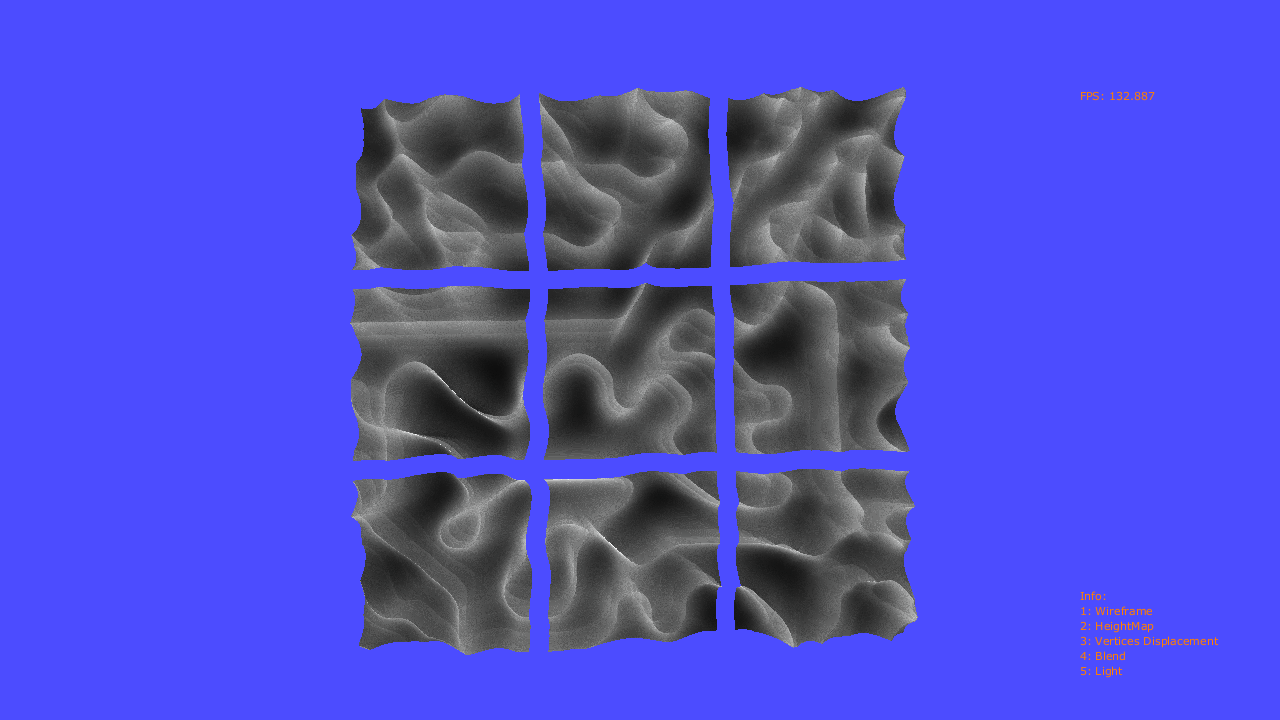
\includegraphics[width=0.6\linewidth]{img/caps/grid.png}}
	\caption{\label{fig:resultados:grid} \emph{Patchs} exibidos em um \emph{grid}.}
\end{figure}

Considerando o usu�rio inicialmente localizado no \emph{patch} central, ao mover-se para um \emph{patch} vizinho, o sistema ir� requisitar a gera�a� de novos \emph{patchs}, vizinhos a aqueles que est�o na borda do grid. O n�mero de vizinhos gerados, bem como a quantidade de vizinhos do \emph{patch} central s�o vari�veis do sistema, podendo ser adaptadas, pelo usu�rio, de acordo com o poder de processamento de sua m�quina.

Para garantir uma visualiza��o fluida do terreno, minimizando as interrup��es com a gera��o, o sistema proposto decidir� qual arquitetura (GPU ou CPU) ser� utilizada na gera��o dos \emph{patchs} a partir de uma vari�vel $\alpha$, que representa a porcentagem de gera��es que ocorrer�o na \emph{GPU}. $1 - \alpha$ representar�, portanto a porcentagem de gera��es na \emph{CPU}.

A Figura \ref{fig:geracao} mostra como se d� o fluxo de gera��o.

\begin{figure}[h]
	\center{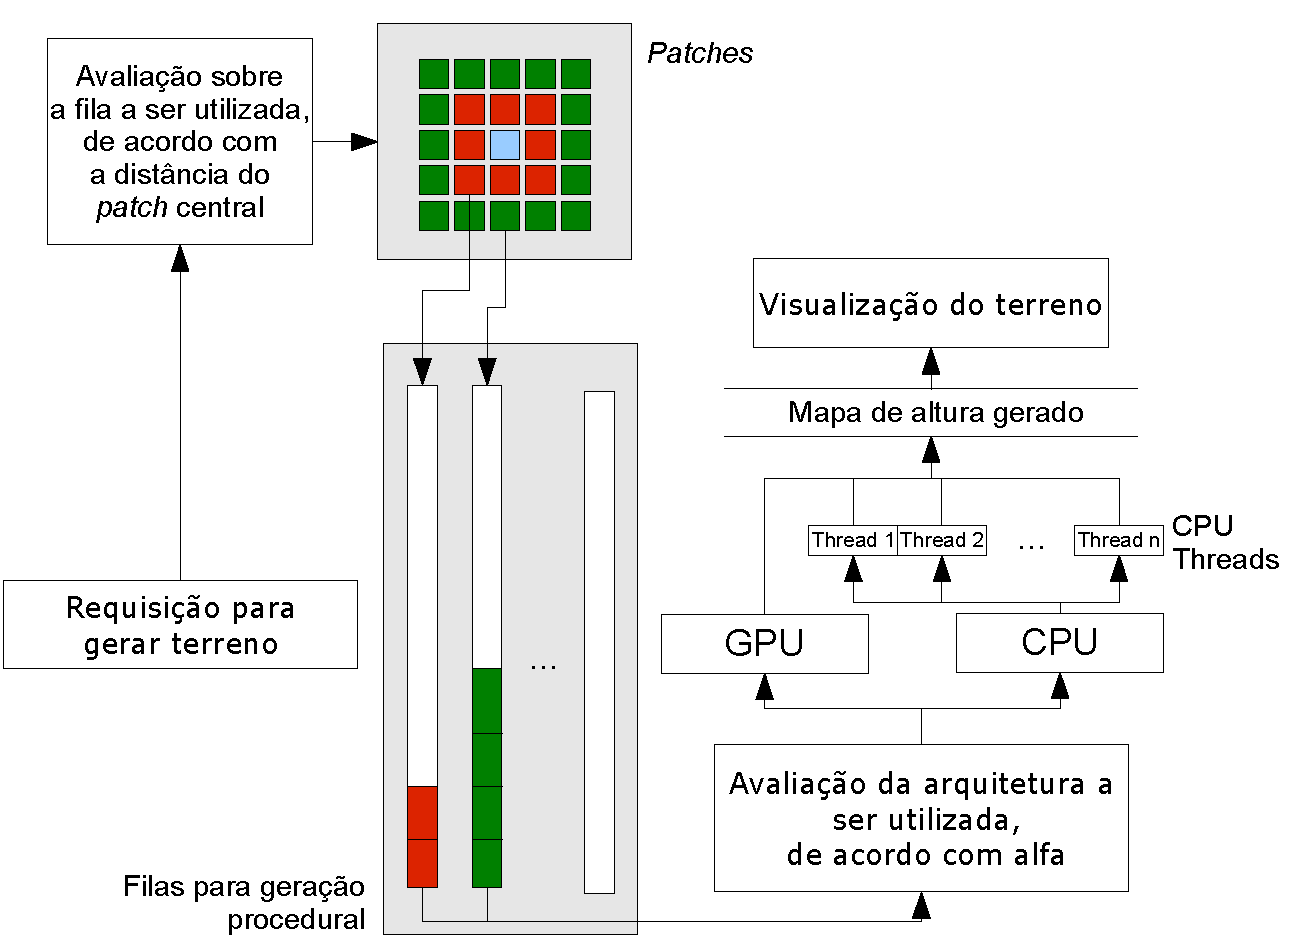
\includegraphics[width=1.0\linewidth]{img/geracao.pdf}}
	\caption{\label{fig:geracao} Fluxo da gera��o procedural.}
\end{figure}


As requisi��es por novos terrenos ser�o adicionadas a uma fila e uma pol�tica \emph{First In, First Out} (FIFO) ser� utilizada para decidir qual terreno ser� gerado. Como � poss�vel ver na Figura \ref{fig:geracao}, o n�mero de filas existentes no sistema ser� igual ao n�mero de vizinhos do \emph{patch} central. Dessa forma, � poss�vel decidir quais terrenos ser�o gerados a partir de sua dist�ncia do \emph{patch} central.

A \emph{thread} principal ficar� encarregada da requisi��o para gerar novos eventos, avalia��o da fila, avalia��o da arquitetura a ser utilizada as chamadas �s fun��es OpenGL. A gera��o na CPU ocorrer� em outras \emph{threads}, n�o a principal.



\subsection{O C�lculo de $\alpha$}

O valor da vari�vel $\alpha$ �, atualmente, uma vari�vel controlada manualmente pelo usu�rio.  A sua varia��o de acordo com a utiliza��o de cada arquitetura ser� um tema a ser abordado em trabalhos futuros.

Atualmente, a maior dificuldade para medir o tempo de gera��o tanto na GPU � a falta de um padr�o nas extens�es dispon�veis em OpenGL. A extens�o \textbf{GL\_EXT\_timer\_query} \cite{timerQuery}, por exemplo, s� est� dispon�vel em placas NVidia, algo que anularia a possibilidade da execu��o deste trabalho em placas ATI.

A utiliza��o de chamadas como \textbf{glFinish()} para sincronizar a CPU e a GPU e assim medir o tempo de gera��o dos terrenos poderia prejudicar a performance do sistema, j� que p�ra a execu��o da CPU enquanto todos os os comandos OpenGL n�o forem executados.

Uma outra op��o para a sincroniza��o seria a extens�o \textbf{GL\_NV\_fence} \cite{nvFence}, que oferece fun��es para sincroniza��o semelhantes ao \textbf{glFinish()} e \textbf{glFlush()}, por�m com um grau maior de controle sobre quais comandos OpenGL dever�o ser executados na chamada. Mais uma vez, por�m, a extens�o n�o est� dispon�vel para placas ATI.

\subsection{Gera��o}
Toda a gera��o dos terrenos na GPU � feita atrav�s de um \emph{fragment shader}, utilizando o ru�do Perlin como foi proposto em \cite{improvedPerlinNoise}. Como toda computa��o de \emph{shaders} fica limitada a geometrias ou texturas, foi preciso renderizar um quadrado utilizando as fun��es OpenGL, para que, dessa forma, fosse poss�vel aplicar os \emph{shaders} �s suas primitivas e iniciar os c�lculos necess�rios. O resultado da gera��o � renderizado em um \emph{framebuffer} \emph{off-screen}, que n�o � exibido na tela, atrav�s da exten��o FBO, que permite criar novos \emph{buffers}.

O c�lculo dos vetores gradientes, necess�rio no ru�do Perlin, � feito na CPU, apenas no in�cio do sistema, e depois � acessado no \emph{fragment shader} como uma textura 2D.

Como o mapa de altura � gerado na GPU, n�o h� qualquer tipo de perda de desempenho com a transfer�ncia entre a mem�ria RAM e a mem�ria da placa de v�deo. Um aspecto importante � que, durante a gera��o do mapa de altura, os valores das normais de cada v�rtice tamb�m s�o calculados.

A gera��o utilizando a CPU � feita utilizando o mesmo algoritmo implementado na GPU. Como o mapa de altura gerado reside na mem�ria principal, sua renderiza��o depender� da transfer�ncia para a mem�ria da placa de v�deo.


\subsection{Visualiza��o}
Com o mapa de altura gerado, o pr�ximo passo � exibir o terreno para o usu�rio, que � feito de forma id�ntica tanto para os terrenos gerados na GPU quanto para os gerados na CPU.

O passo inicial � a gera��o de uma malha (conjunto de v�rtices) de tamanho pr�-determinado, como mostra a Figura \ref{fig:malha}.

\begin{figure}[h]
	\center{
\includegraphics[width=0.5\linewidth]{img/caps/malha.png}}
	\caption{\label{fig:malha} Malha inicial para visualiza��o dos terrenos.}
\end{figure}

A malha � gerada de tal forma que um n�mero maior de v�rtices est� concentrado no centro. Quanto maior a dist�ncia, menor o n�mero de v�rtices presentes. Isto propicia uma maneira r�pida e f�cil de implementar um n�vel de detalhamento (quanto maior a dist�ncia do centro, menor ser� a necessidade de se renderizar o terreno em alta fidelidade).

Como a malha � gerada apenas uma �nica vez (no in�cio da execu��o), n�o � preciso criar repetidas malhas a medida que o jogador percorre o terreno. Apenas os mapas de altura de cada \emph{patch} s�o trocados, como mostra a Figura \ref{fig:texturas}

\begin{figure}[h]
	\center{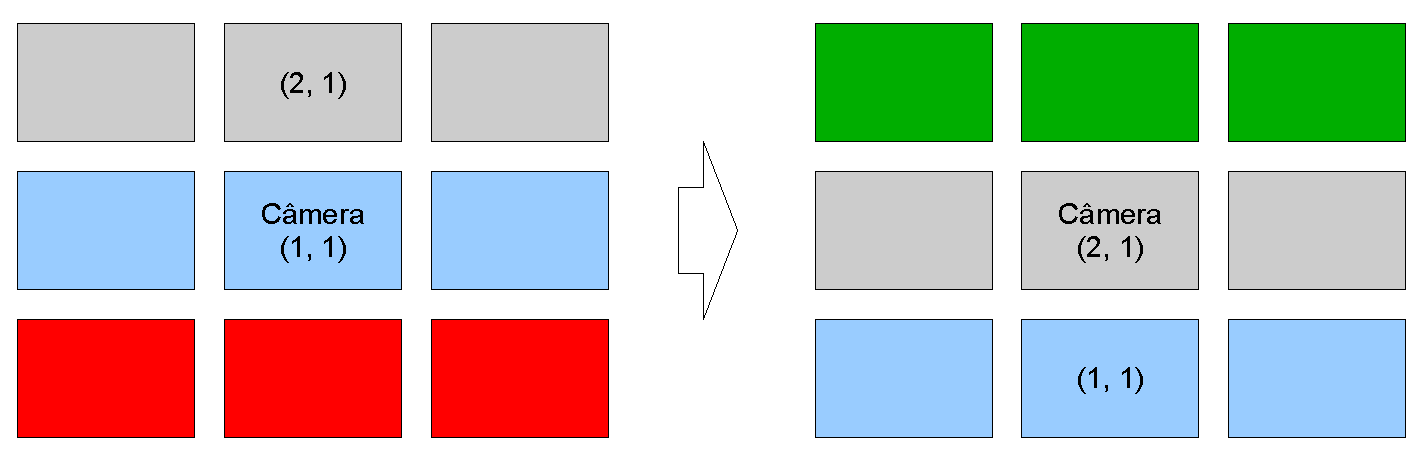
\includegraphics[width=0.8\linewidth]{img/texturas.pdf}}
	\caption{\label{fig:texturas} Movimenta��o da c�mera para um outro \emph{patchs}.}
\end{figure}

Na Figura \ref{fig:texturas} � poss�vel notar o deslocamento dos mapas de textura quando a c�mera move para o \emph{patch} superior ao (1,1). Para que haja uma transi��o, uma matriz de transla��o, com valores iguais ao tamanho do \emph{patch}, � feita e multiplicada � matriz respons�vel por renderizar todas as primitivas, resultando na transla��o de todos os \emph{patchs}. 

Este m�todo diminuiu a necessidade de implementa��o de um algoritmo de n�vel de detalhe mais robusto. Al�m disso, como sabemos o n�mero de v�rtices antecipadamente, a performance do aplicativo tem uma menor chance de sofrer quedas bruscas de rendimento.




\begin{figure*}[t]
	\center{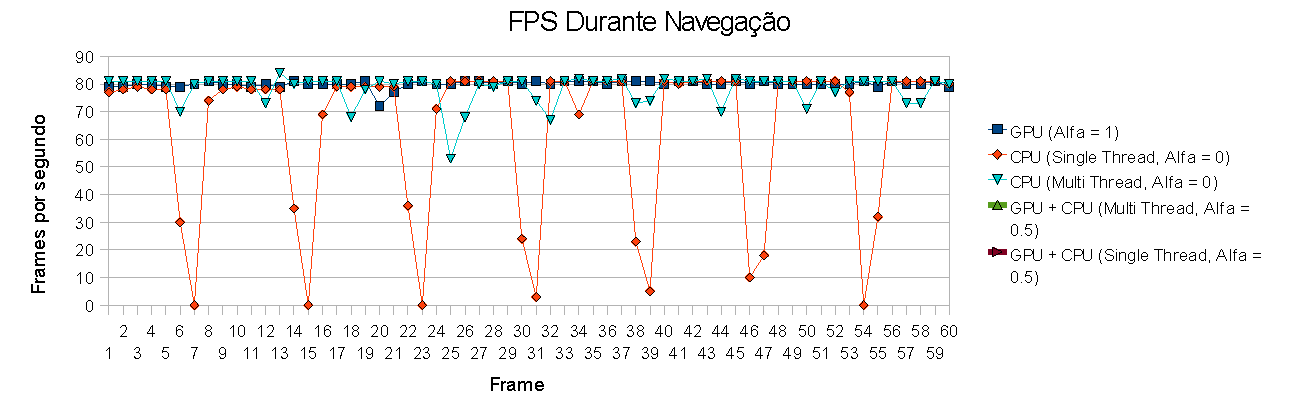
\includegraphics[width=1.0\linewidth]{img/fps.pdf}}
	\caption{\label{fig:fps} Gr�fico com o FPS na navega��o pelo mundo durante 60 segundos.}
\end{figure*}

\begin{figure}[h]
	\center{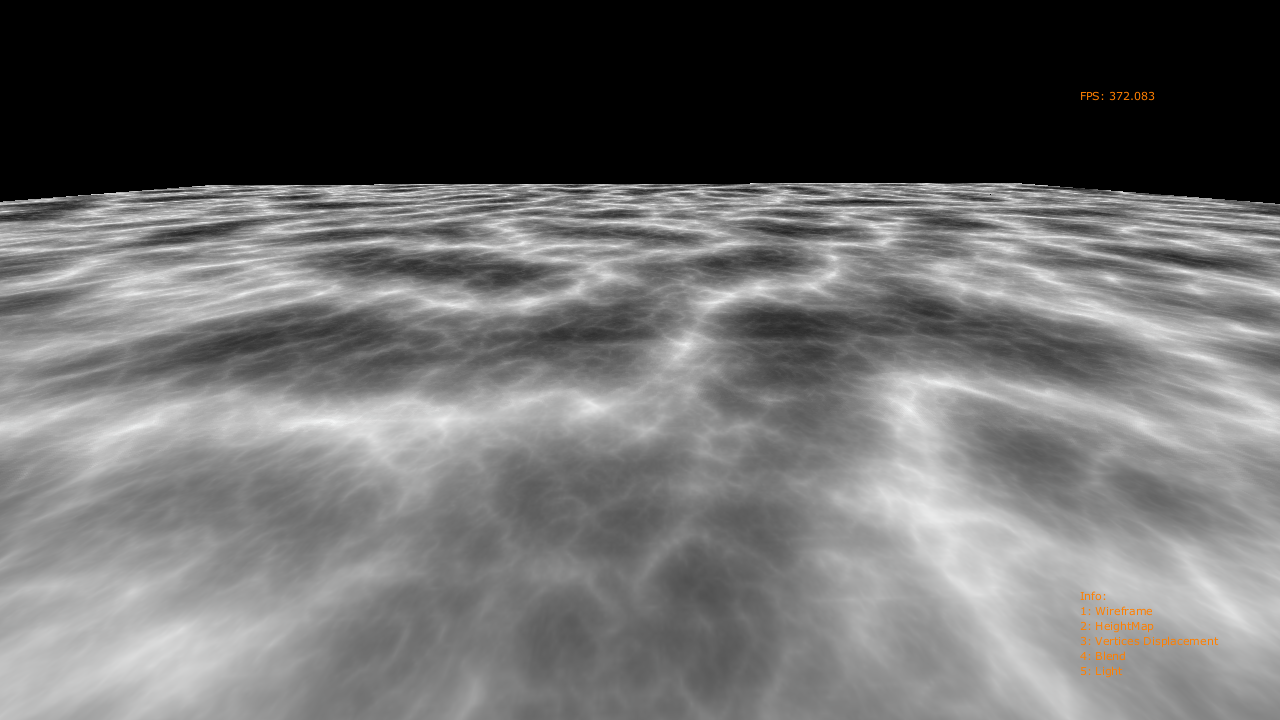
\includegraphics[width=1.0\linewidth]{img/caps/heightmap.png}}
	\caption{\label{fig:heightmap} Mapa de altura aplicado a um quadrado.}
\end{figure}

\begin{figure}[h]
	\center{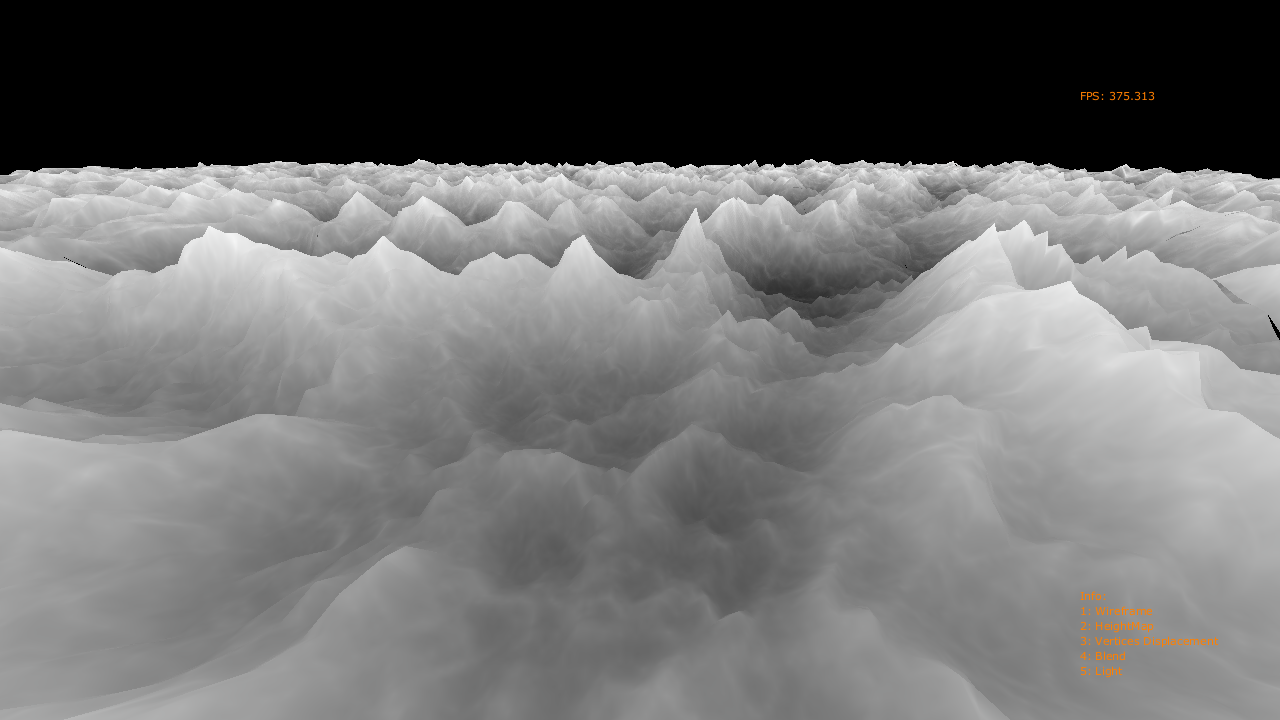
\includegraphics[width=1.0\linewidth]{img/caps/deslocamento.png}}
	\caption{\label{fig:deslocamento} Mapa de altura aplicado a um quadrado, deslocando a altura.}
\end{figure}

\begin{figure}[h]
	\center{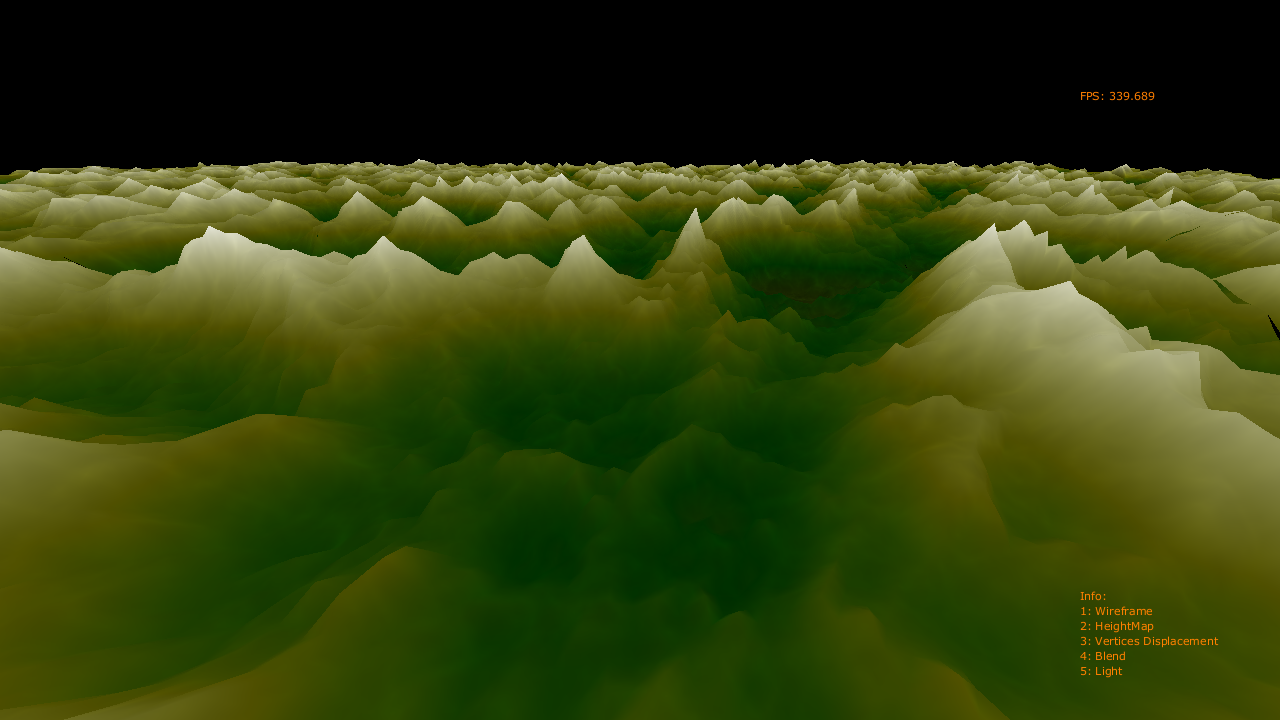
\includegraphics[width=1.0\linewidth]{img/caps/blend.png}}
	\caption{\label{fig:blend} Mapa de altura aplicado a um quadrado, deslocando a altura, e com texturas.}
\end{figure}

\begin{figure}[h]
	\center{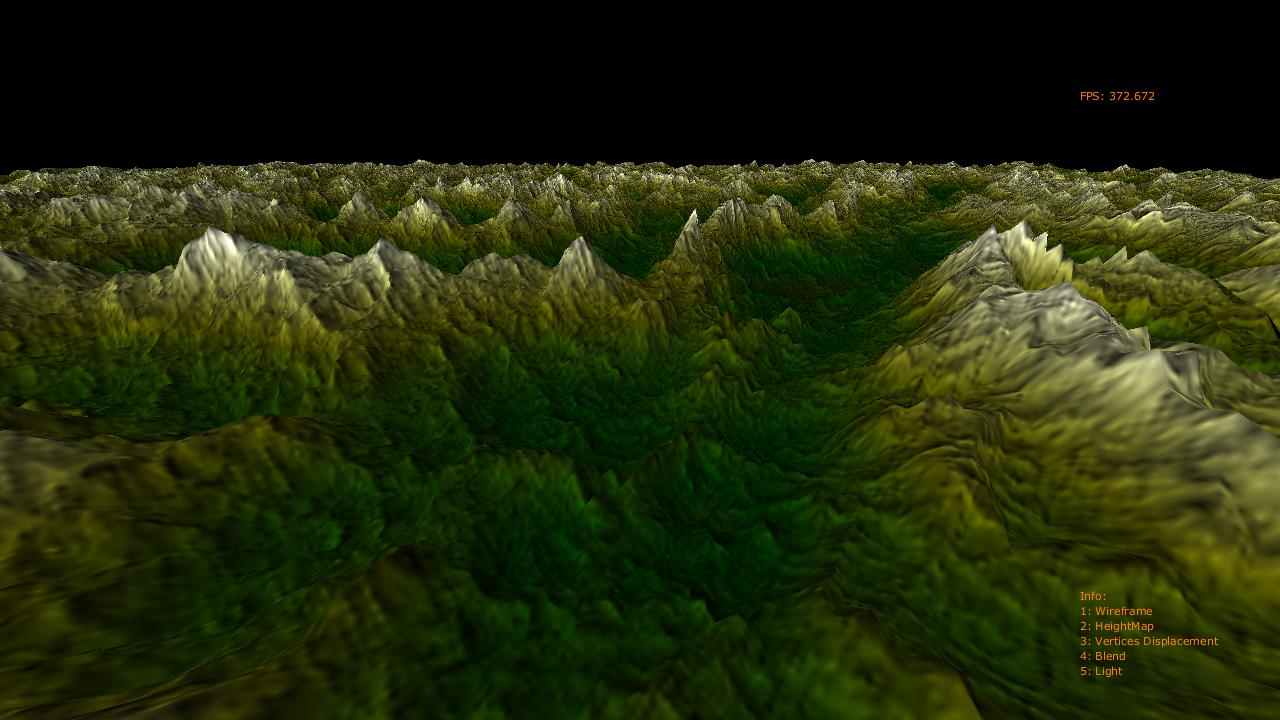
\includegraphics[width=1.0\linewidth]{img/caps/luz.png}}
	\caption{\label{fig:luz} Mapa de altura aplicado a um quadrado, deslocando a altura, com texturas, e ilumina��o.}
\end{figure}
\chapter{IMPLEMENTA��O}
\label{implementacao}

Os conhecimentos adquiridos ao longo desse trabalho permitiram a cria��o de um sistema capaz de gerar terrenos procedurais tanto na GPU quanto na CPU, e tamb�m permite a navega��o do usu�rio por tal terreno. Na Se��o \ref{sistema} ser� apresentado uma vis�o geral do sistema. As Se��es \ref{geracao} e \ref{visualizacao} mostrar�o como os terrenos s�o gerados e visualizados.



\section{Vis�o Geral do Sistema}
\label{sistema}

O sistema implementado neste trabalho teve como principal objetivo permitir a gera��o procedural de terrenos tanto na GPU quanto na CPU. A Figura \ref{fig:bibliotecas} apresenta as camadas do sistema, destacando as bibliotecas utilizadas (como � explicado a seguir).

\begin{figure}[H]
	\center{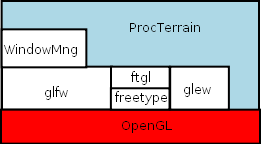
\includegraphics[width=0.3\linewidth]{img/bibliotecas.png}}
	\caption{\label{fig:bibliotecas} Camadas do sistema.}
\end{figure}

\begin{itemize}
	\item {\bf OpenGL}: \emph{API} gr�fica utilizada para a renderiza��o.
	\item {\bf glew}: Biblioteca para carregamento de extens�o do \emph{OpenGL}.
	\item {\bf glfw}: Biblioteca que facilita o tratamento de entradas e tamb�m cria��o de janelas.
	\item {\bf ftgl}: Biblioteca para a renderiza��o de textos.
	\item {\bf FreeType}: Biblioteca para renderiza��o de textos (depend�ncia do \emph{ftgl}).
	\item {\bf WindowMng}: Camada respons�vel por criar a tela e tratar os eventos de entrada.
	\item {\bf ProcTerrain}: Camada respons�vel por gerar e exibir os terrenos.
\end{itemize}

As camadas \emph{WindowMng} e \emph{ProcTerrain} foram implementadas neste trabalho. O \emph{WindowMng} tem como prop�sito simular a camada de um aplicativo gr�fico gen�rico (\emph{game}, simulador, etc.); desta forma, o sistema poder� ser posteriormente adaptado para funcionar em conjunto com outros aplicativos que possam ser desenvolvidos.

A Figura \ref{fig:arquitetura} apresenta em detalhes os m�dulos presentes nas camadas \emph{WindowMng} e \emph{ProcTerrain}. A seguir, uma explica��o sobre cada um dos m�dulos.

\begin{figure}[H]
	\center{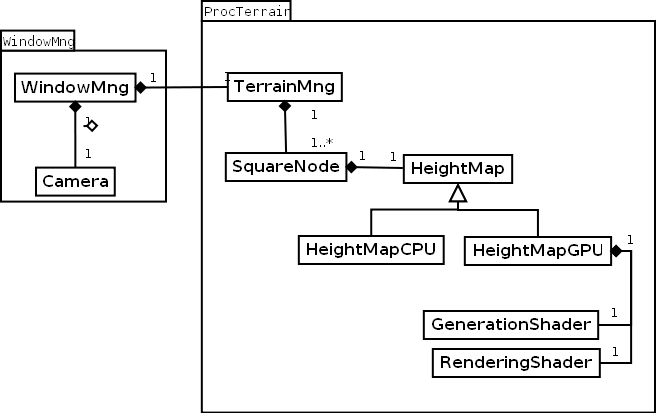
\includegraphics[width=0.5\linewidth]{img/arquitetura.png}}
	\caption{\label{fig:arquitetura} Diagrama com as principais classes do sistema implementado.}
\end{figure}

\begin{itemize}
	\item {\bf WindowMng}: Respons�vel por simular um aplicativo gr�fico gen�rico, e chamar os devidos \emph{callbacks} do pacote \emph{ProcTerrain}.
	\item {\bf Camera}: M�dulo que implementa uma c�mera controlada pelo jogador e navegando pelo mundo.
	\item {\bf TerrainMng}: M�dulo respons�vel por gerar e controlar os terrenos.
	\item {\bf SquareNode}: Nodo que representa uma fatia (\emph{patch}) do terreno.
	\item {\bf HeightMap}, {\bf HeightMapCPU} e {\bf HeightMapGPU}: M�dulos que implementam os mapas de altura dos terrenos gerados na CPU ou na GPU.
	\item {\bf GenerationShader}: \emph{Shader} respons�vel pela gera��o dos terrenos.
	\item {\bf RenderingShader}: \emph{Shader} respons�vel pela renderiza��o dos terrenos.
\end{itemize}


\section{Gera��o do Terreno}
\label{geracao}
Nesta se��o, ser� abordada a implementa��o da gera��o de terrenos, tanto na GPU, quanto na CPU. Os dois t�m, em comum, o algoritmo usado para a gera��o (\emph{Ridged multifractal noise}, descrito na Se��o \ref{ridged}).

O terreno geral � dividido em terrenos menores (chamados \emph{patchs}), como mostra o \emph{grid} da Figura \ref{fig:resultados:grid}:

\begin{figure}[H]
	\center{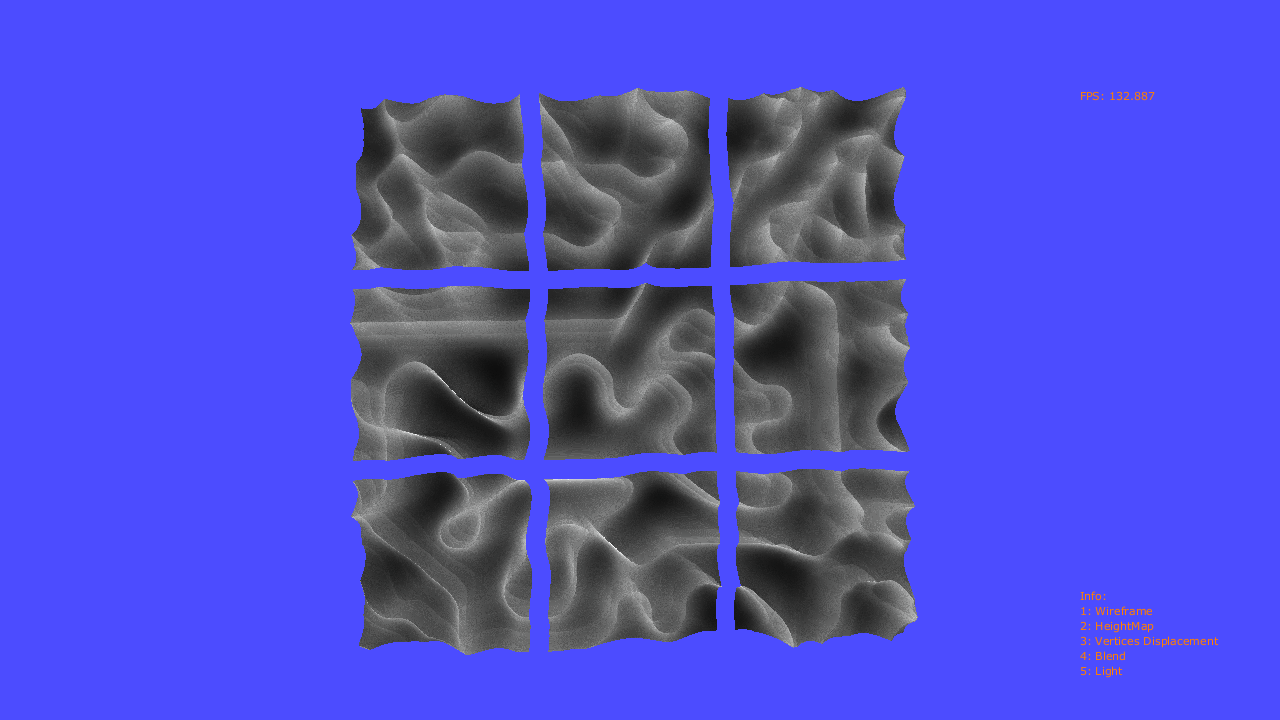
\includegraphics[width=0.5\linewidth]{img/caps/grid.png}}
	\caption{\label{fig:resultados:grid} \emph{Patchs} exibidos em um \emph{grid}.}
\end{figure}

Considerando o usu�rio inicialmente localizado no \emph{patch} central, ao mover-se para um \emph{patch} vizinho, o sistema ir� requisitar a gera�a� de novos \emph{patchs}, vizinhos a aqueles que est�o na borda do grid. O n�mero de vizinhos gerados, bem como a quantidade de vizinhos do \emph{patch} central s�o vari�veis do sistema, podendo ser adaptadas, pelo usu�rio, de acordo com o poder de processamento de sua m�quina.


\subsection{Gera��o do Terreno na GPU}
Toda a gera��o dos terrenos na GPU � feita atrav�s de um \emph{fragment shader}. Como toda computa��o de \emph{shaders} fica limitada a geometrias ou texturas, foi preciso renderizar um quadrado utilizando as fun��es OpenGL, para que, dessa forma, fosse poss�vel aplicar os \emph{shaders} �s suas primitivas e iniciar os c�lculos necess�rios. O resultado da gera��o � renderizado em um \emph{framebuffer} \emph{off-screen}, que n�o � exibido na tela, atrav�s da exten��o FBO, que permite criar novos \emph{buffers}.

O c�lculo dos vetores gradientes, necess�rio no ru�do Perlin, � feito na CPU, apenas no in�cio do sistema, e depois � acessado no \emph{fragment shader} como uma textura 2D.

A Figura \ref{fig:resultados:heightmap} apresenta o resultado da gera��o, visto como um mapa de altura.

\begin{figure}[H]
	\center{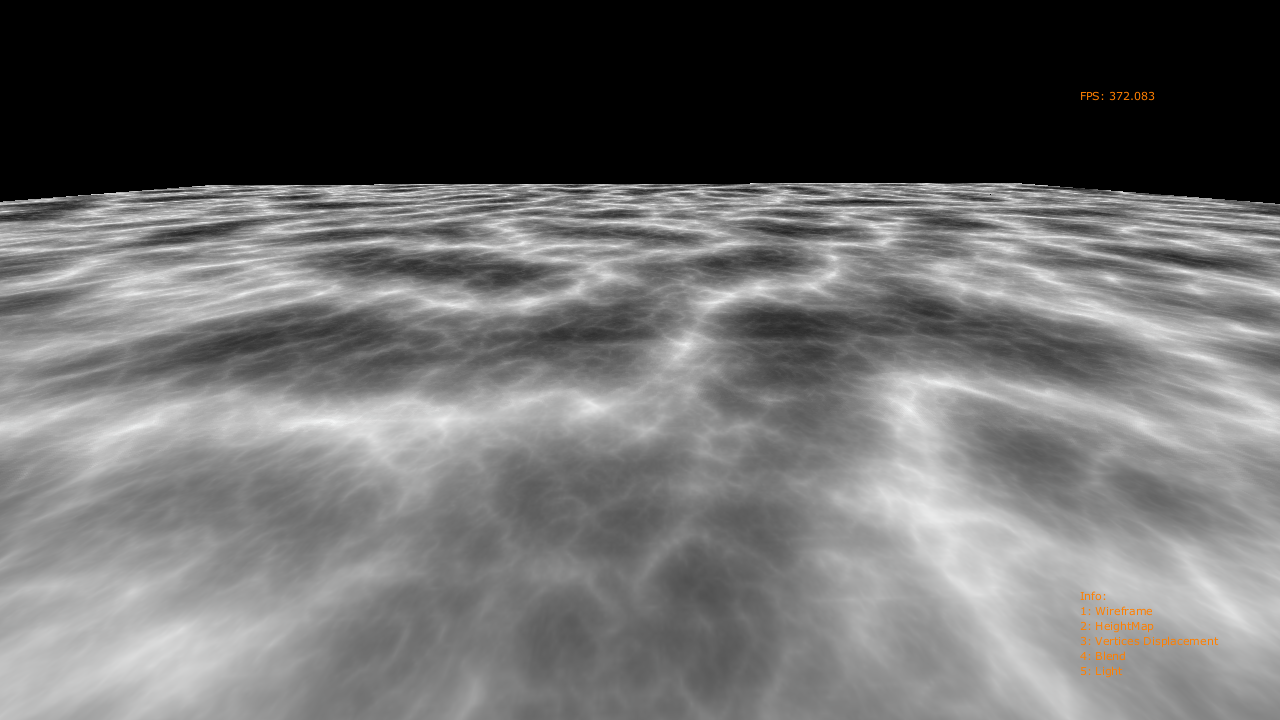
\includegraphics[width=0.5\linewidth]{img/caps/heightmap.png}}
	\caption{\label{fig:resultados:heightmap} Mapa de altura gerado pelo \emph{shader}.}
\end{figure}

Como o mapa de altura � gerado na GPU, n�o h� qualquer tipo de perda de desempenho com a transfer�ncia entre a mem�ria RAM e a mem�ria da placa de v�deo. Um aspecto importante � que, durante a gera��o do mapa de altura, os valores das normais de cada v�rtice tamb�m s�o calculados.



\subsection{Gera��o do Terreno na CPU}
A gera��o na CPU � feita de maneira tradicional. Uma matrix com o tamanho da textura do mapa de altura � preenchida de acordo com o algoritmo \emph{Ridged multifractal noise}, e posteriormente enviada para a mem�ria da GPU.



\section{Visualiza��o do Terreno}
\label{visualizacao}
Com o mapa de altura gerado, o pr�ximo passo � exibir o terreno para o usu�rio, que � feito de forma id�ntica tanto para os terrenos gerados na GPU quanto para os gerados na CPU.

O passo inicial � a gera��o de uma malha (conjunto de v�rtices) de tamanho pr�-determinado, como mostra a Figura \ref{fig:malha}.

\begin{figure}[H]
	\center{
\includegraphics[width=0.5\linewidth]{img/caps/malha.png}}
	\caption{\label{fig:malha} Malha inicial para visualiza��o dos terrenos.}
\end{figure}

A malha � gerada de tal forma que um n�mero maior de v�rtices est� concentrado no centro. Quanto maior a dist�ncia, menor o n�mero de v�rtices presentes. Isto propicia uma maneira r�pida e f�cil de implementar um n�vel de detalhamento (quanto maior a dist�ncia do centro, menor ser� a necessidade de se renderizar o terreno em alta fidelidade).

Como a malha � gerada apenas uma �nica vez (no in�cio da execu��o), n�o � preciso criar repetidas malhas a medida que o jogador percorre o terreno. Apenas os mapas de altura de cada \emph{patch} s�o trocados, como mostra a Figura \ref{fig:texturas}

\begin{figure}[H]
	\center{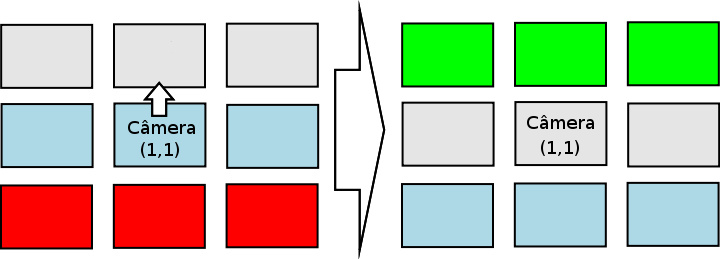
\includegraphics[width=0.8\linewidth]{img/texturas.png}}
	\caption{\label{fig:texturas} Movimenta��o da c�mera para um outro \emph{patchs}.}
\end{figure}

Na Figura \ref{fig:texturas} � poss�vel notar o deslocamento dos mapas de textura quando a c�mera move para o \emph{patch} superior ao (1,1). Para que haja uma transi��o, uma matriz de transla��o, com valores iguais ao tamanho do \emph{patch}, � feita e multiplicada � matriz \emph{MODELVIEW}, respons�vel por renderizar todas as primitivas, resultando na transla��o de todos os \emph{patchs}. 

Este m�todo diminuiu a necessidade de implementa��o de um algoritmo de n�vel de detalhe mais robusto. Al�m disso, como sabemos o n�mero de v�rtices antecipadamente, a performance do aplicativo tem uma menor chance de sofrer quedas bruscas de rendimento.

Ap�s a gera��o dos v�rtices, as texturas com os mapas de altura gerados proceduralmente s�o aplicados � malha. Um \emph{vertex shader} l� ent�o a altura presente no mapa e desloca a posi��o de \emph{z} do v�rtice correspondente na malha.

A cor de cada fragmento � calculada a partir de quatro diferentes texturas, simulando areia, grama, pedras e neve. A participa��o de cada uma delas na cor final depender� da altura do v�rtice correspondente do fragmento. Para pontos mais altos, a textura de neve ser� predominante e, pontos mais baixos, ser�o cobertos pela textura de grama. Entre esses pontos, haver� uma mistura das outras texturas.




\section{Testes}
\label{testes}

Para comprovar a efici�ncia do sistema, foi feito um teste que consiste na navega��o por um trajeto constante pelo terreno gerado proceduralmente, durante 30 segundos. O teste foi executado para cinco valores diferentes de $\alpha$: 1.0 (gera��o totalmente na GPU), 0.7, 0.4, 0.0 (gera��o totalmente na CPU).


\begin{figure}[h]
	\center{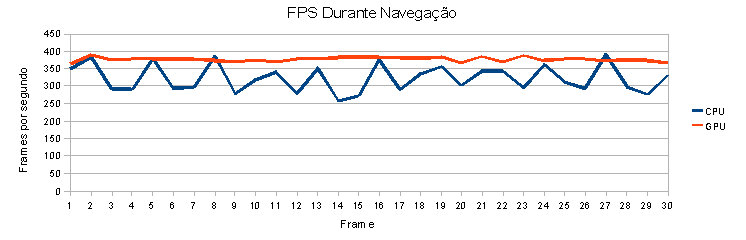
\includegraphics[width=0.9\linewidth]{img/tempoFPS.png}}
	\caption{\label{fig:fps} Gr�fico com o FPS na navega��o pelo mundo durante 30 segundos.}
\end{figure}
\section{Conclus�o e Trabalhos Futuros}
\label{conclusao}

Os resultados obtidos na gera��o procedural de terrenos na GPU mostram o poder de processamento das placas gr�ficas em rela��o �s CPU. A op��o de se gerar nas duas arquiteturas mostra-se promissora, principalmente considerando a utiliza��o do sistema acoplado a um \emph{game} ou simulador. Como haver� inevitavelmente outras tarefas sendo executadas (\emph{path-finding}, sombras, HDR), a possibilidade de se migrar a carga de trabalho envolvida na gera��o procedural pode ser bastante vantajosa.

Como trabalho futuro, espera-se encontrar uma estrat�gia eficiente para o c�lculo de $\alpha$. Dessa forma, a gera��o procedural poder� ser balanceada automaticamente entre as diferentes arquiteturas utilizadas (CPU e GPU).

O sistema foi implementado sempre tendo em mente a sua utiliza��o acoplada a outras aplicativos. Assim, adot�-lo em um \emph{game} ou simulador demandaria pouco esfor�o.

\bibliographystyle{sbgames}
\bibliography{paper}

%

\begin{figure*}[t]
	\center{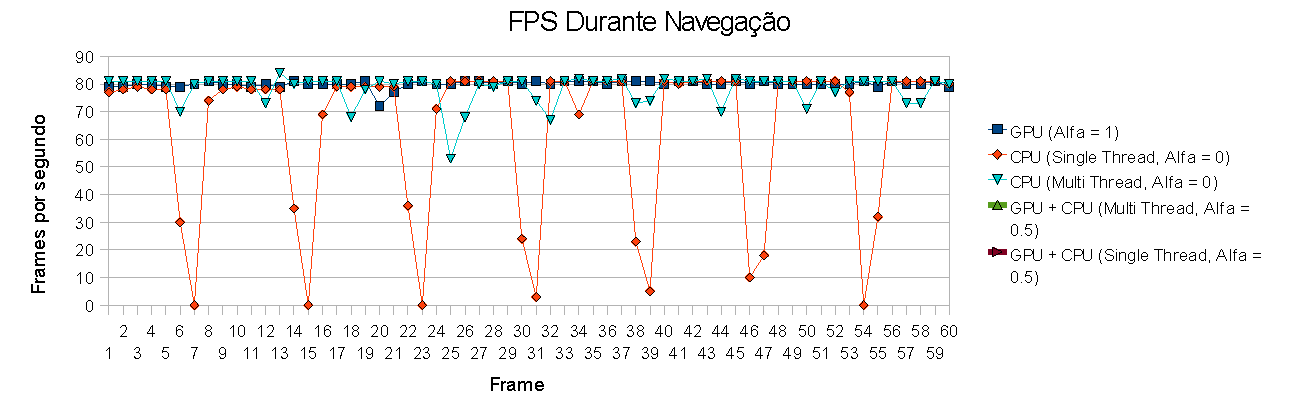
\includegraphics[width=1.0\linewidth]{img/fps.pdf}}
	\caption{\label{fig:fps} Gr�fico com o FPS na navega��o pelo mundo durante 60 segundos.}
\end{figure*}

\begin{figure}[h]
	\center{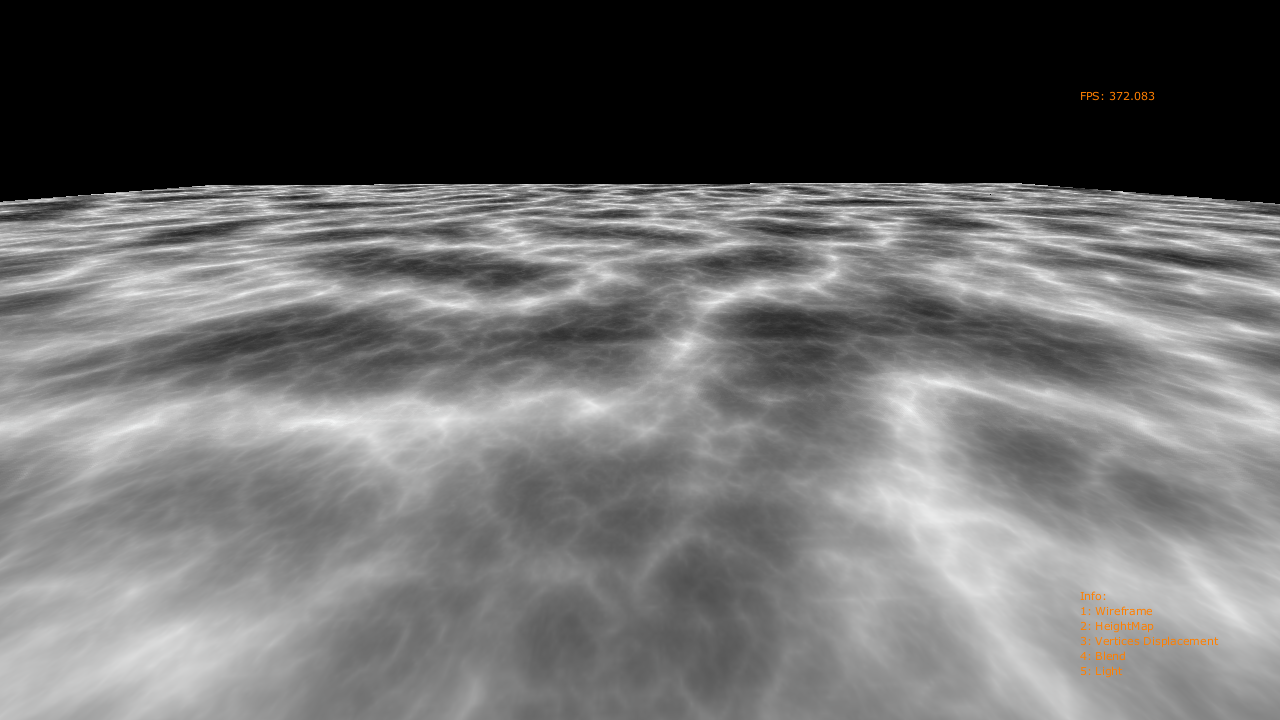
\includegraphics[width=1.0\linewidth]{img/caps/heightmap.png}}
	\caption{\label{fig:heightmap} Mapa de altura aplicado a um quadrado.}
\end{figure}

\begin{figure}[h]
	\center{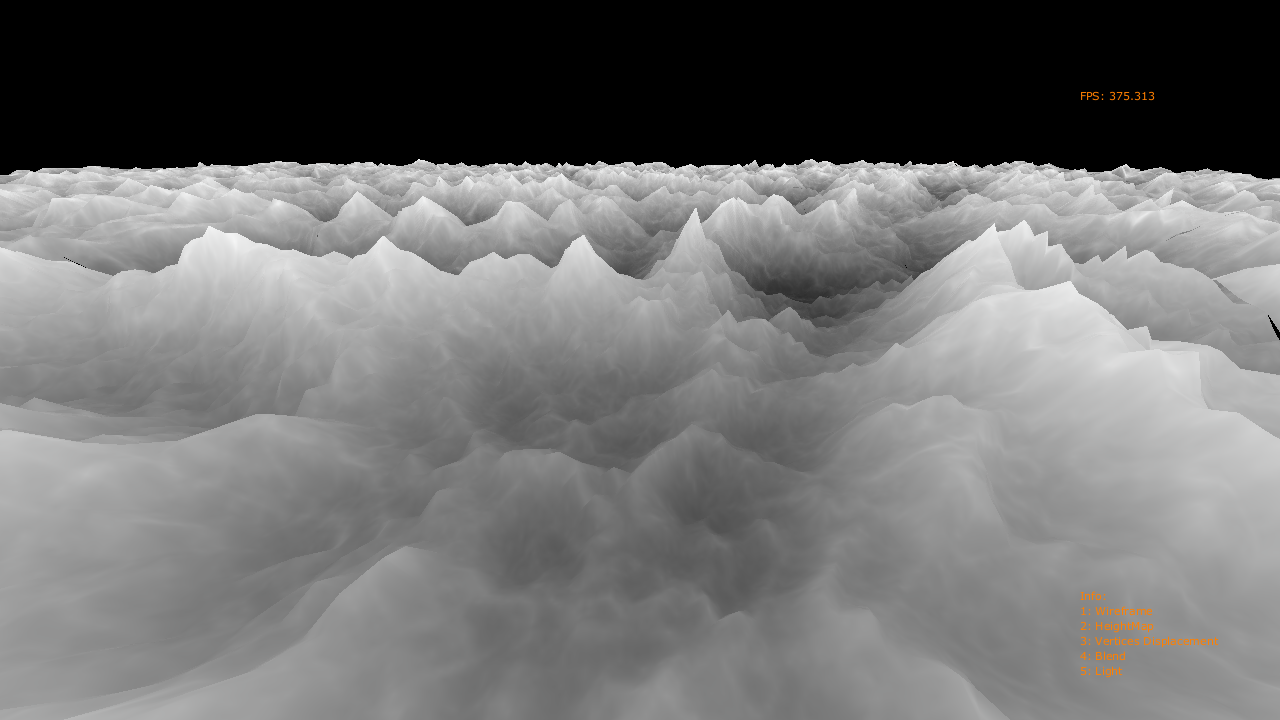
\includegraphics[width=1.0\linewidth]{img/caps/deslocamento.png}}
	\caption{\label{fig:deslocamento} Mapa de altura aplicado a um quadrado, deslocando a altura.}
\end{figure}

\begin{figure}[h]
	\center{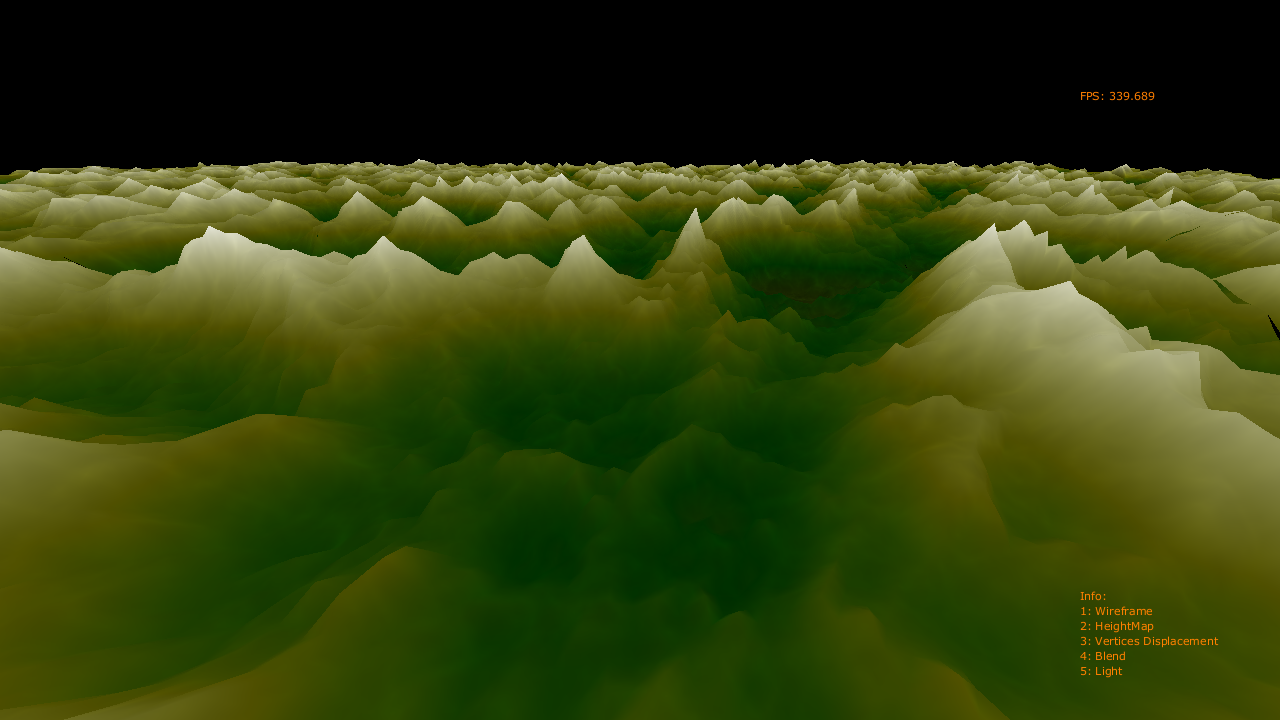
\includegraphics[width=1.0\linewidth]{img/caps/blend.png}}
	\caption{\label{fig:blend} Mapa de altura aplicado a um quadrado, deslocando a altura, e com texturas.}
\end{figure}

\begin{figure}[h]
	\center{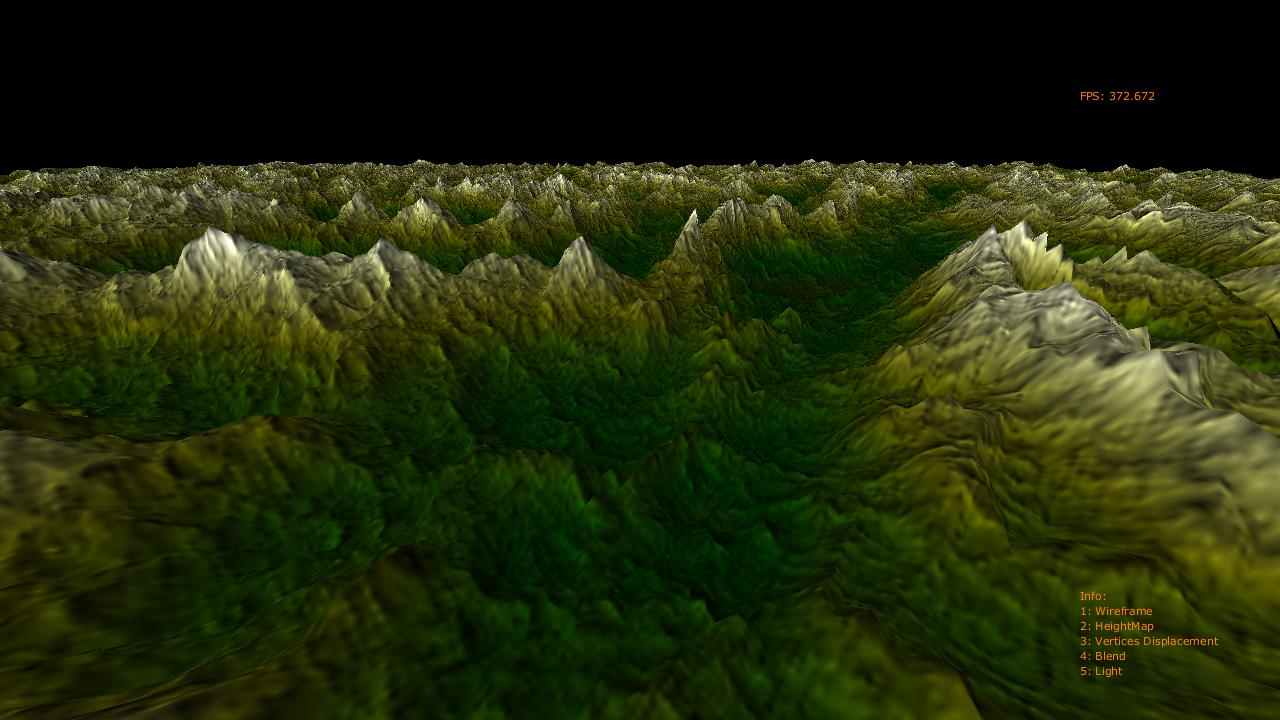
\includegraphics[width=1.0\linewidth]{img/caps/luz.png}}
	\caption{\label{fig:luz} Mapa de altura aplicado a um quadrado, deslocando a altura, com texturas, e ilumina��o.}
\end{figure}

\end{document}
